\chapter{Lösungsansatz}\label{chp:loesungsansatz}

Um besser den Lösungsansatz zu verstehen, wird erstmal der Ablauf von der Erstellung von Anforderung bis zu einem Testfall erläutert. Als erstes wird in DOORS alle schon vordefinierte Anforderungen eingetragen (siehe \ref{sec:DOORS}). In diesen Anforderung können Parameter vorkommen, die für die Testfälle relevant sind. Die Parameter werden als folgendes in einer Anforderung eintragen:\\

\begin{center}
\#param [\textit{Parametername}]\\
\#param [max\_Geschwindigkeit]\\
Das Auto hat eine Maximalgeschwindigkeit von \#param[max\_geschwindigkeit] km/h
\end{center}

Die Parameter sind in einer Parameter-Tabelle definiert, wo die jeweilige Parameterwerte eingetragen werden. Der Grund, dass es eine extra Tabelle für Parameter gibt, kommt daher, dass die Parameter in der Regel pro Variante verschiedene Werte annehmen. Zum Beispiel beträgt die maximale Geschwindigkeit bei einem Cabrio 150 km/h  und bei einem Kombi 200 km/h. Dank dieser Tabelle werden die Varianten (Cabrio und Kombi) die richtige Parameterwerte zugewiesen.\\

Da Parameterwerte und Varianten schon verlinkt sind, müssen die Anforderungen, die Parametern beinhalten, mit der Parametertabelle manuell verlinkt werden. Wenn dieser Vorgang abgeschlossen ist, kann über die TESTONA Oberfläche die Verbindung zu DOORS aufgebaut werden um die nötigen Informationen zu importieren. Es wird davon ausgegangen, dass der Tester bereits ein Klassifikationsbaum passend zum testenden Produkt und die dazu gehörige Anforderungen erstellt hat. Jetzt können die in DOORS definierte Varianten importiert. Als erstes muss der Tester die Baumelemente der richtigen Variante zuordnen (durch ein Ausschlussverfahren, es wird angenommen, dass alle Baumelemente in alle Varianten gültig sind). 


%#######################################################################################
%#######################################################################################
\newpage
\section{Parameterspeicherung}
\paragraph{}
 
Um die Parameter erfolgreich in TESTONA zu speichern, müssen diese aus DOORS importiert werden und aus den Anforderungen gelesen werden. Durch eine gezielte Anfrage an DOORS, über eine Java API, kann die Parametertabelle in TESTONA geladen werden. Die darin bestimmte Beziehungen (Parameterwert zu Variante) müssen fest in die TESTONA Datei gespeichert werden, damit diese auch ohne eine DOORS Verbindung zur Verfügung steht. Als erstes werden die Parameterwerte in Objekte gespeichert und einen \textit{Tag} (Kennzeichen) gegeben und nach Programmende in die TESTONA Datei im XML Format gespeichert. Dank des \textit{Tags} kann beim Programmstart wieder der Parameterwert gelesen werden und währen das Programm ausgeführt wird, Änderungen vornehmen.\\

Einer der Besonderheiten von MERAN in Verbindung mit TESTONA ist, dass Anforderungen and Baumelemente per Drag\&Drop verknüpft werden können. Mit dieser Funktion muss der Tester die Anforderung mit einem dazu gehörigen Baumelement verknüpfen (auslösendes Ereignis der Parameterspeicherung). Damit das Programm die Aktion des Benutzer mitbekommen, wird an dieser Stelle ein \textit{Listener} implementiert. Der \textit{Listener} bekommt verschiedene Nachrichten von Ereignisse die gefiltert werden müssen. Wenn die Nachricht empfangen wird, dass eine Anforderung an ein Baumelement verknüpft wurde, muss eine zu programmierende Methode das Anforderungstext von dieses Baumelement lesen und nach Parameter suchen. Als erstes wird davon ausgegangen, dass ein Baumelement nur eine Anforderung beinhalten kann und eine Anforderung nur ein Parameter beinhaltet. Wird in die gelesene Anforderung ein Parameter gefunden, so müssen die möglichen Werten dieses Parameters aus die DOORS Parameter-Tabelle gelesen und gespeichert werden. An dieser Stelle beginnt die Parameterspeicherung.\\

Für die Parameterspeicherung ergeben sich zwei Lösungswege. Die erste Lösung lautet, die Parametertabelle beim importieren der Anforderung gleich in TESTONA zu speichern. Diese Lösung hat den Vorteil, dass später eine Verbindung zu DOORS nicht mehr notwendig ist. Somit muss während der Parametersuche nach eine Verbindung mit DOORS nicht geprüft werden, oder die Verbindung muss nicht wieder aufgebaut werden. Das heißt der Benutzer muss sich nur einmal mit DOORS Verbinden und kann in der Zukunft problemlos die Anforderungen an Baumelement verlinken und zugleich werden die Parameter gelesen und gespeichert. Der Nachteil ist, dass möglicherweise unnötige Daten in TESTONA gespeichert werden.\\

Die zweite Lösung ist der Gegensatz zu die erste. Hier werden jeweils nur die Daten gespeichert, die der Benutzer im Moment verbraucht. Wird eine Anforderung an einem Baumelement verlinkt, so muss eine Verbindung zu DOORS aufgebaut werden (wenn sie nicht vorhanden ist) und die Parametertabelle aufrufen und in TESTONA speichern. Der große Nachteil dieser Lösung ist, dass der Benutzer möglicherweise nicht eine Verbindung zu DOORS aufbauen kann (Server nicht Vorhanden, keine Zugriff Möglichkeiten, etc.). Welcher der beiden Lösungen implementiert wird, wird erst genauer analysiert und ist auch abhängig von den Anforderungen verschiedener Kunden und wie diese TESTONA anwenden. Die implementierte Lösung wird in Kapitel \ref{chp:systementwurf} vorgestellt und begründet.\\


Sind die Parameterwerte in TESTONA vorhanden, müssen diese an der richtigen Variante noch zugeordnet werden. Dafür ist vorgesehen, dass der Parameterwert als Eigenschaft des Baumelementes gespeichert wird (als ein \textit{Tag} Objekt). Die Darstellungsstruktur für die Variantenansicht ist etwa folgendermaßen definiert:\\

\begin{figure}[h!]
  \begin{center}
    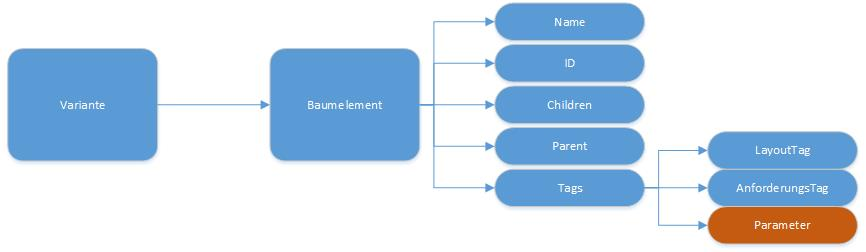
\includegraphics[scale=0.5]{4_1_UML_Var_TreeItem_Properties.jpg}
  		  \caption{Darstellung der TESTONA Objekte für die Parameterspeicherung}
     \label{ttn.depencyRulesEdit}
  \end{center}
\end{figure}


Somit kann jetzt in TESTONA ein Parameterwert mit einer Variante und ein Baumelement verknüpft werden. Als Ergebnis werden folgenden Beziehungen erwartet:

\begin{center}
\textbf{Anforderung 1: }Das Auto hat eine Maximalgeschwindigkeit von \#param[max\_Geschwindigkeit] km/h.
\end{center}

\begin{table}[h]
\begin{center}
	\begin{tabular}{|l||c|c|}
	 \hline
	 Variante &Maximalgeschwindigkeit &Anforderung\\
	 \hline\hline
	 Cabrio   &150                      & 1\\
	 \hline
	 Kombi    &200                      & 1\\
	 \hline
	 Limo     &250                      & 1\\
	 \hline
	\end{tabular}
	
	\caption{Beispiel für die Zuordnung zwischen Varianten und Parameterwert aus einer Anforderung}
	\label{table:4TestCases}
\end{center}
\end{table}

Wenn ein Baumelement verschiedene Anforderungen beinhaltet, mit verschiedene Parameter, wird die aktive Variante entscheiden, welches Parameter ausgewertet wird. Um genauer diesen Fall zu verstehen, sind folgende Bäume, wo ......\\

TODO, Beispiel mit Baumbilder


%#######################################################################################
%#######################################################################################
\newpage
\section{Visualisierung}
\paragraph{}
%1.2 Wenn der Tester die Ansicht zwischen Varianten ändert, muss der Wert hinter dem Parameter auf die jeweilige Variante aktualisiert werden (maximale Geschwindigkeit von Cabrio = x, Limo = y, Kombi = z).

% Als Ergebnis soll bei der Änderung der Variantenansicht, auch  geändert werden. Ist die Variante \textit{Cabrio} aktiv, so muss das Baumelement mit die maximalen Türanzahl der Wert zwei anzeigen. Wird die Variantenansicht geändert auf die Variante \textit{Kombi}, so muss das Baumelement der Wert fünf anzeigen.

Wenn die Beziehungen zwischen Varianten, Parameter und Anforderungen erfolgreich entstanden sind, können jetzt die gespeicherte Parameterwerte angezeigt werden. Hier ist gefordert, dass wenn der Benutzer die Variantenansicht ändert (durch Betätigung an der Benutzeroberfläche) die Beschriftung (\textit{Label}) des Baumelements (Maximaleschwindigkeit von Generic = X, Cabrio = 150, Kombi = 200) aktualisiert werden.\\



\begin{figure}[h!]
  \begin{center}
    
\includegraphics{4_2_Change_Var_Generic.png}
    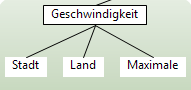
\includegraphics[scale=0.8]{4_2_Change_Var_Generic_Tree.png}
  		  \caption{Aktive Variante Generic (default)}
     \label{ttn.depencyRulesEdit}
  \end{center}
\end{figure}

\begin{figure}[h!]
  \begin{center}
    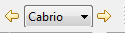
\includegraphics{4_2_Change_Var_Cabrio.png}
    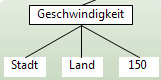
\includegraphics[scale=0.9]{4_2_Change_Var_Cabrio_Tree.png}
  		  \caption{Aktive Variante Cabrio}
     \label{ttn.depencyRulesEdit}
  \end{center}
\end{figure}

\begin{figure}[h!]
  \begin{center}
    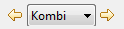
\includegraphics{4_2_Change_Var_Kombi.png}
    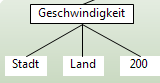
\includegraphics[scale=0.9]{4_2_Change_Var_Kombi_Tree.png}
  		  \caption{Aktive Variante Kombi}
     \label{ttn.depencyRulesEdit}
  \end{center}
\end{figure}

Dafür muss ein \textit{Listener} beim Ändern der Ansicht eine Methode aufrufen, die sich um das aktualisieren der Werte und die Darstellung des Baumelements aktualisiert. Die Methode muss die im Baumelement gespeicherte \textit{Parameter-Tags} lesen und die richtig Parameterwerte (abhängig von der aktiven Variante) im das \textit{Label} schreiben.

%#######################################################################################
%#######################################################################################
\newpage
\section{Testgültigkeit}
\paragraph{}
%Innerhalb einer Variante auf Testfallduplikate überprüfen

%#######################################################################################
%#######################################################################################
\newpage
\section{Optimierungskriterien}
\paragraph{}
%Testablauf optimieren in Betrachtung auf die Varianten und mögliche Testduplikate

%#######################################################################################
%#######################################################################################
\newpage
\section{Benutzeroberfläche}
\paragraph{}

%Um die Handhabung der Varianten bezogen auf die Testfälle und die Testgenerierung benutzerfreundlicher
%und effizienter zu gestalten, soll die Benutzung des Variantenmanagements durch
%einen Testingenieur untersucht werden. Resultierend aus den erworbenen Erkenntnissen wird das
%Lösungsdesign für eine Erweiterung des bestehenden Variantenmanagements in TESTONA konzipiert.

%nach besprechen mit kollegen keine änderung nötig erstmal \\